% Energy reconstruction section should have the following sections:
% Shower Reconstruction (Inlucding resoltuion, validation with pi0)
% track reconstruction (Length based methodology, resolution)
%	- Hadronic energy reconstruction (All tracks in a selected neutrino interaction)
% Neutrino Energy Reconstruction

\section{Energy reconstruction}\label{sec:energyreco}
\subsection{Scope of the reconstruction}
In this analysis we restrict ourselves to the measurement of the deposited energy in the TPC of the visible particles in the final state of the neutrino interaction. Our signal will have in its final state, by definition, one electron and at least one proton, with no other visible particles. The energy of the electron will be measured by converting the hit charge of all the shower-like objects into deposited energy, as described in Section \ref{sec:showerenergy}. The energy of the protons, instead, can be measured by converting the track length of the reconstructed tracks into deposited energy, using the tabulated stopping power of protons in the liquid argon, with the procedure described in \ref{sec:protonenergy}.


\subsection{Electron energy reconstruction and calibration}\label{sec:showerenergy}
The reconstructed energy $E_{reco}^{e}$ of a shower-like object is measured converting the charge of the associated hits into deposited energy in the TPC. It is calculated by multiplying the reconstructed charge ($e^{-}_{reco}$) from hits associated with the reconstructed shower by the calibration factor measured in \cite{michel}:
\begin{equation}
\frac{E_{reco}^{e} \mathrm{(MeV)}}{e^-} = 1.01\frac{e^-}{e^{-}_{reco}} \times \frac{23.6~\mathrm{eV}}{e^-} \times 10^{-6} \frac{\mathrm{eV}}{\mathrm{MeV}} \times \frac{1}{R},\label{eq:calib}
\end{equation}
where:
\begin{itemize}

\item the correction factor $1.01\frac{e^-}{e^{-}_{reco}}$ is obtained measuring the true number of collected electrons $e^{-}$ on the wires using a sample of stopping muons, fitting the $dE/dx$ vs. residual range to values for argon as tabulated by the PDG \cite{pdg},
\item $\frac{23.6~\mathrm{eV}}{e^-}$ is the work function for ionizing an argon atom \cite{workfunction},
\item $R = 0.62$ is the recombination factor obtained with the Modified Box Model \cite{boxmodel}.
\end{itemize}
Figure \ref{fig:ecalib} shows the calibration slope necessary to convert the electron reconstructed energy $E_{reco}^{e}$ into true electron energy $E_{true}^{e}$. It has been obtained using only the hits reconstructed in the collection plane. 
The reconstructed energy is obtained summing the hits energy from each reconstructed shower matched to the true electron. The true electron and the reconstructed showers are required to be fully contained within the fiducial volume. Since the reconstructed energy distributions in each true energy bin is asymmetrical, the data points are obtained fitting a Gaussian around the peak of the distribution.
A linear fit of the data points gives:
\begin{equation}
E_{reco}^{e} = 0.78~E^{e} - 0.02~\mathrm{GeV}.
\end{equation}

\begin{figure}[htbp]
\centering
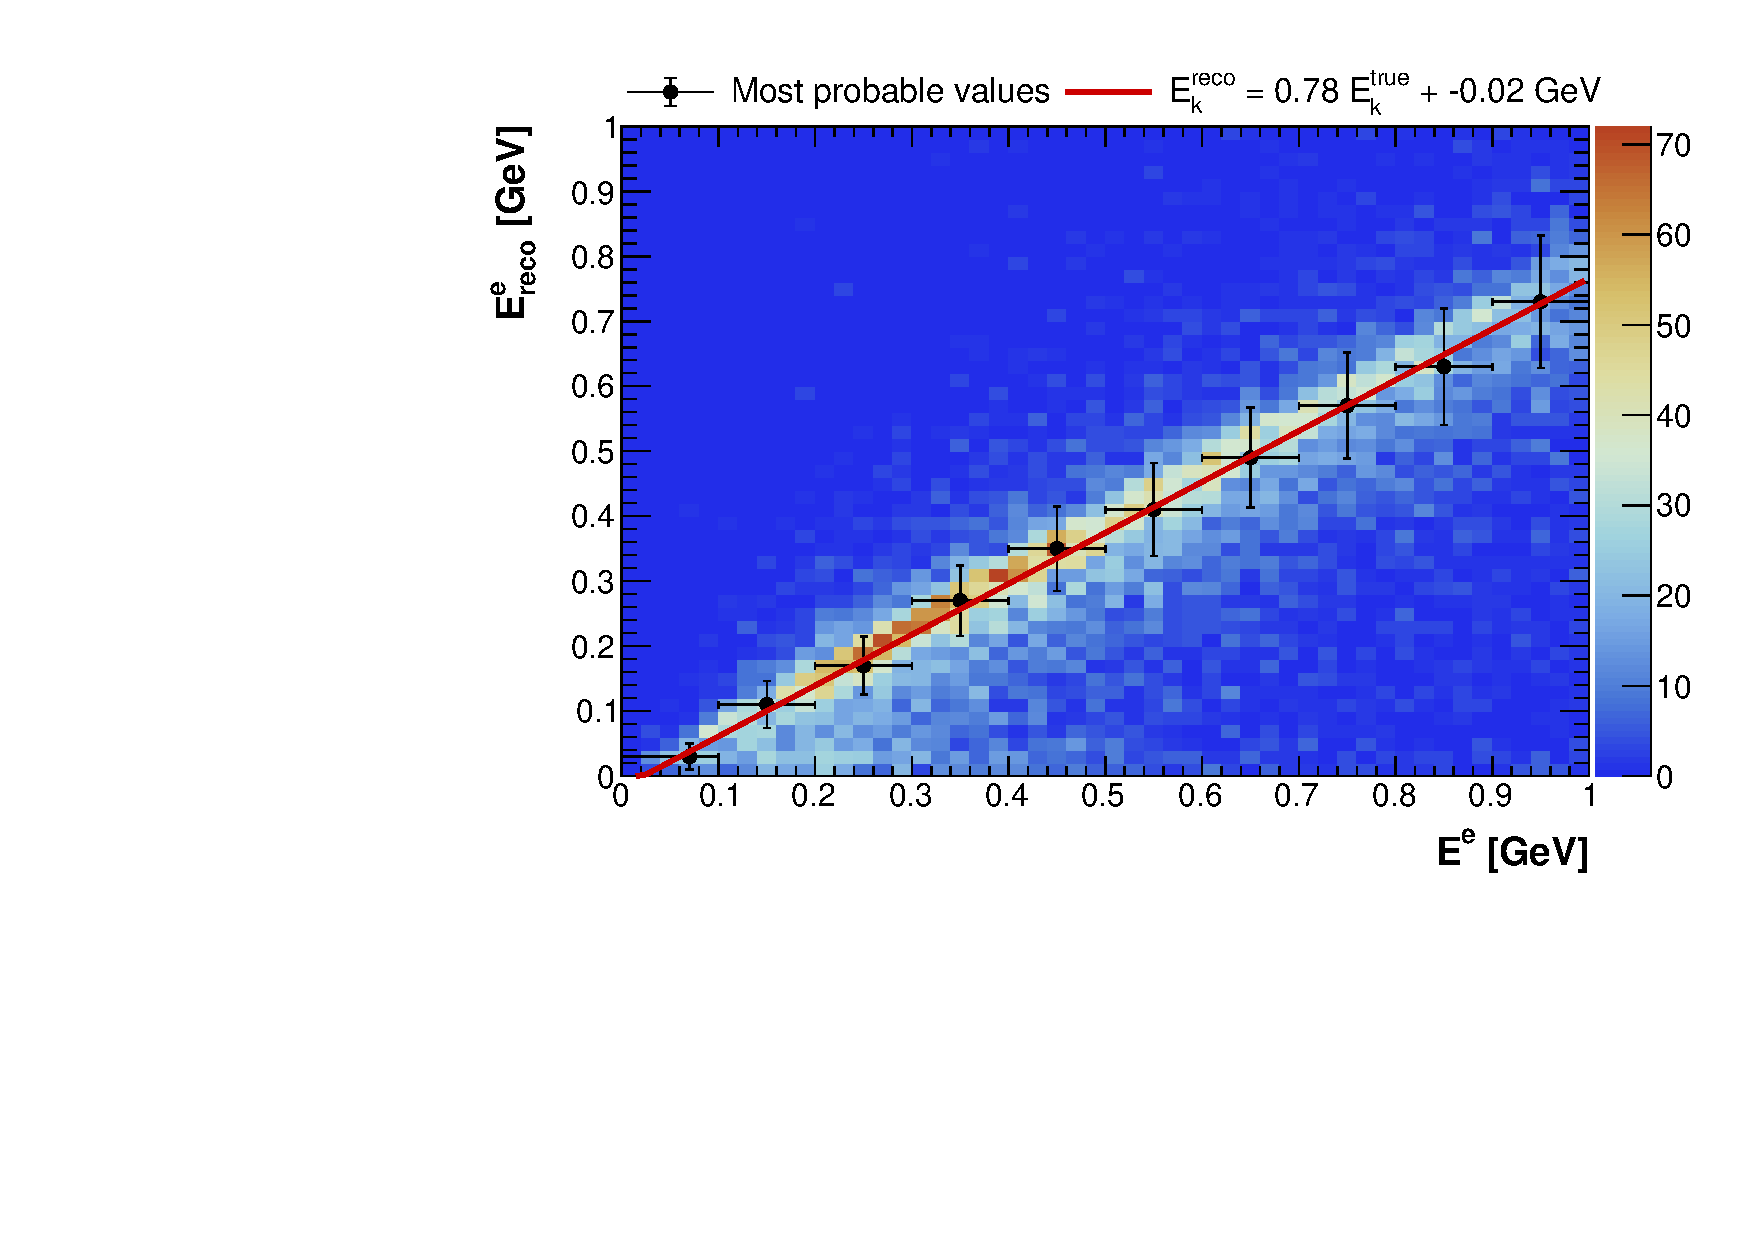
\includegraphics[width=0.65\columnwidth]{figures/ecalib.pdf}
\caption{Bi-dimensional histogram of true electron energy $E^{e}$ vs. reconstructed electron energy $E_{reco}^{e}$. Black points are obtained measuring the most probable value of the $E_{reco}^{e}$ distribution for each $E^{e}$ bin.}
\label{fig:ecalib}
\end{figure}



\subsubsection{\texorpdfstring{$\pi^0$}{pi0} mass peak}

CC$\pi^0$ events have been studied in order to validate the energy scale and reconstruction in the low-energy region in data as well as in the Monte Carlo. There is no aim for an analysis in the CC$\pi^0$ channel. Instead the purpose is to exploit a pure sample of $\pi^0$ decays, which can be used as standard candle to validate the energy reconstruction.
The samples which have been used are:
\begin{itemize}
  \item Data: hand scanned CC$\pi^0$ sample, which has been already used in \cite{caratelli}.
  \item Monte Carlo: BNB intrinsic $\nu_{\mu}$ with cosmic rays.
\end{itemize}
The optical selection, described in Section \ref{sec:optical_pre_cuts}, and the topological pre-selection, described in Section \ref{sec:topological_pre_selection}, are applied to both samples.
An additional set of generator level requirements is applied to the Monte Carlo sample, in order to identify CC$\pi^0$ using truth information:
\begin{itemize}
    \item The selected neutrino candidate must be matched to the true neutrino interaction.
    \item The interaction must be a charged current interaction.
    \item Exactly one $\pi^0$ must be present in the final state.
\end{itemize}
Subsequently events are required to have at least two reconstructed showers, both with hits on the collection plane. The second requirement is meant to remove events with null shower energy, as the energy is computed from the collection plane only. The energy of the showers is calibrated as shown previously in Section \ref{sec:showerenergy}, deriving correction factors from electrons-matched-showers using the simulation, as shown in Figure \ref{fig:ecalib}.
The $\pi^0$ candidate is computed starting from the two most energetic showers. The distribution of the number of reconstructed showers in each event is shown in the left plot in Figure \ref{fig:mc_mass_e2} for data and Monte Carlo.

As there are many events with more than two showers, about two thirds in data and one half in Monte Carlo, a simple re-clustering of the energy is performed. It is meant to recover the energy from broken showers. The two most energetic showers are considered. Then, the energy of any additional shower is summed to the closest in angle among the two most energetic showers. The direction of the two most energetic showers is not modified in this process. The mass is computed from the two most energetic showers, with the energy corrected after the re-clustering, as:
\[ M = \sqrt{E_1 E_2 (1 - \cos\theta)} \]
where $E_1$ and $E_2$ are the energies of the most and the second most energetic showers, respectively. $\theta$ is the 3-D angle between the directions of the two showers.

\begin{figure}[!htbp]
\centering
\begin{minipage}{0.49\columnwidth}
  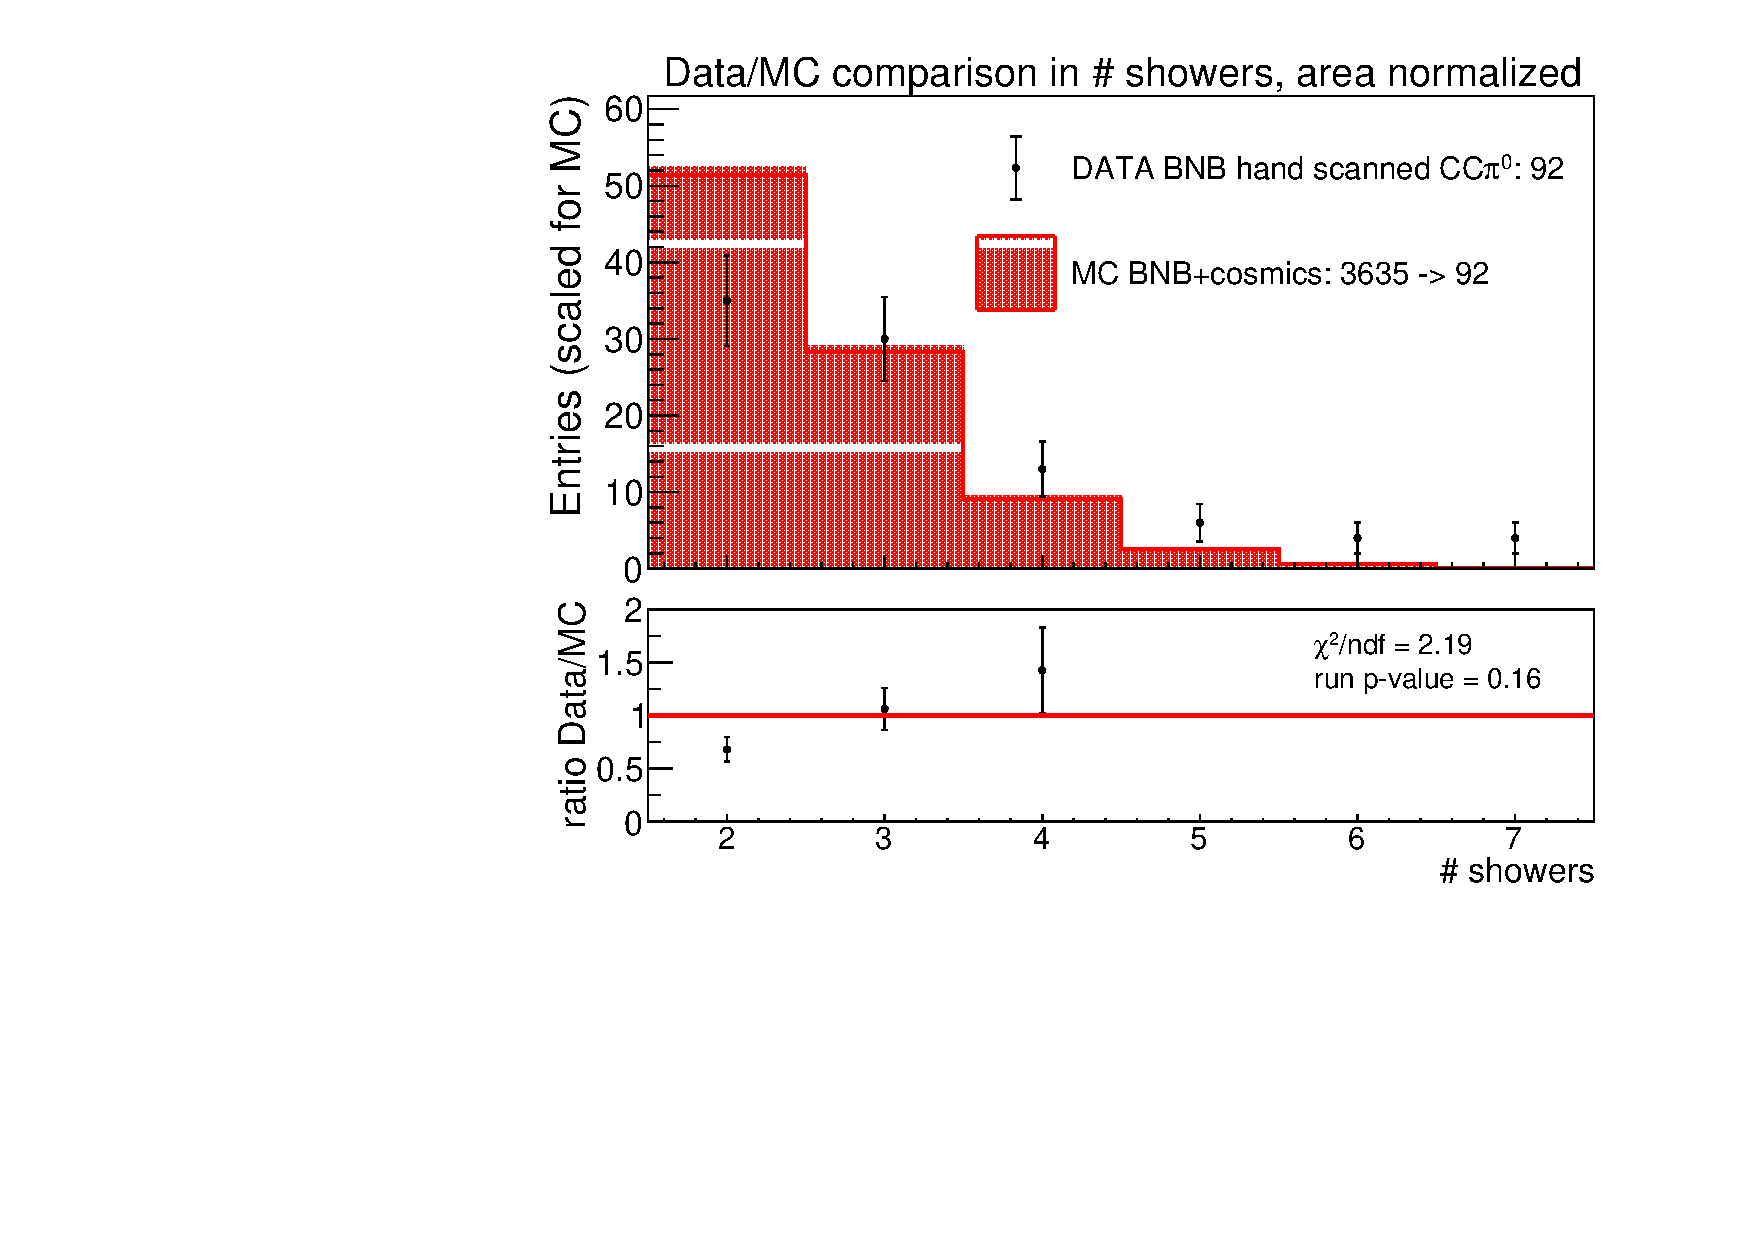
\includegraphics[width=0.99\columnwidth]{figures/n_showers_data_MC_comparison_mod.pdf}
\end{minipage}
\begin{minipage}{0.49\columnwidth} 
  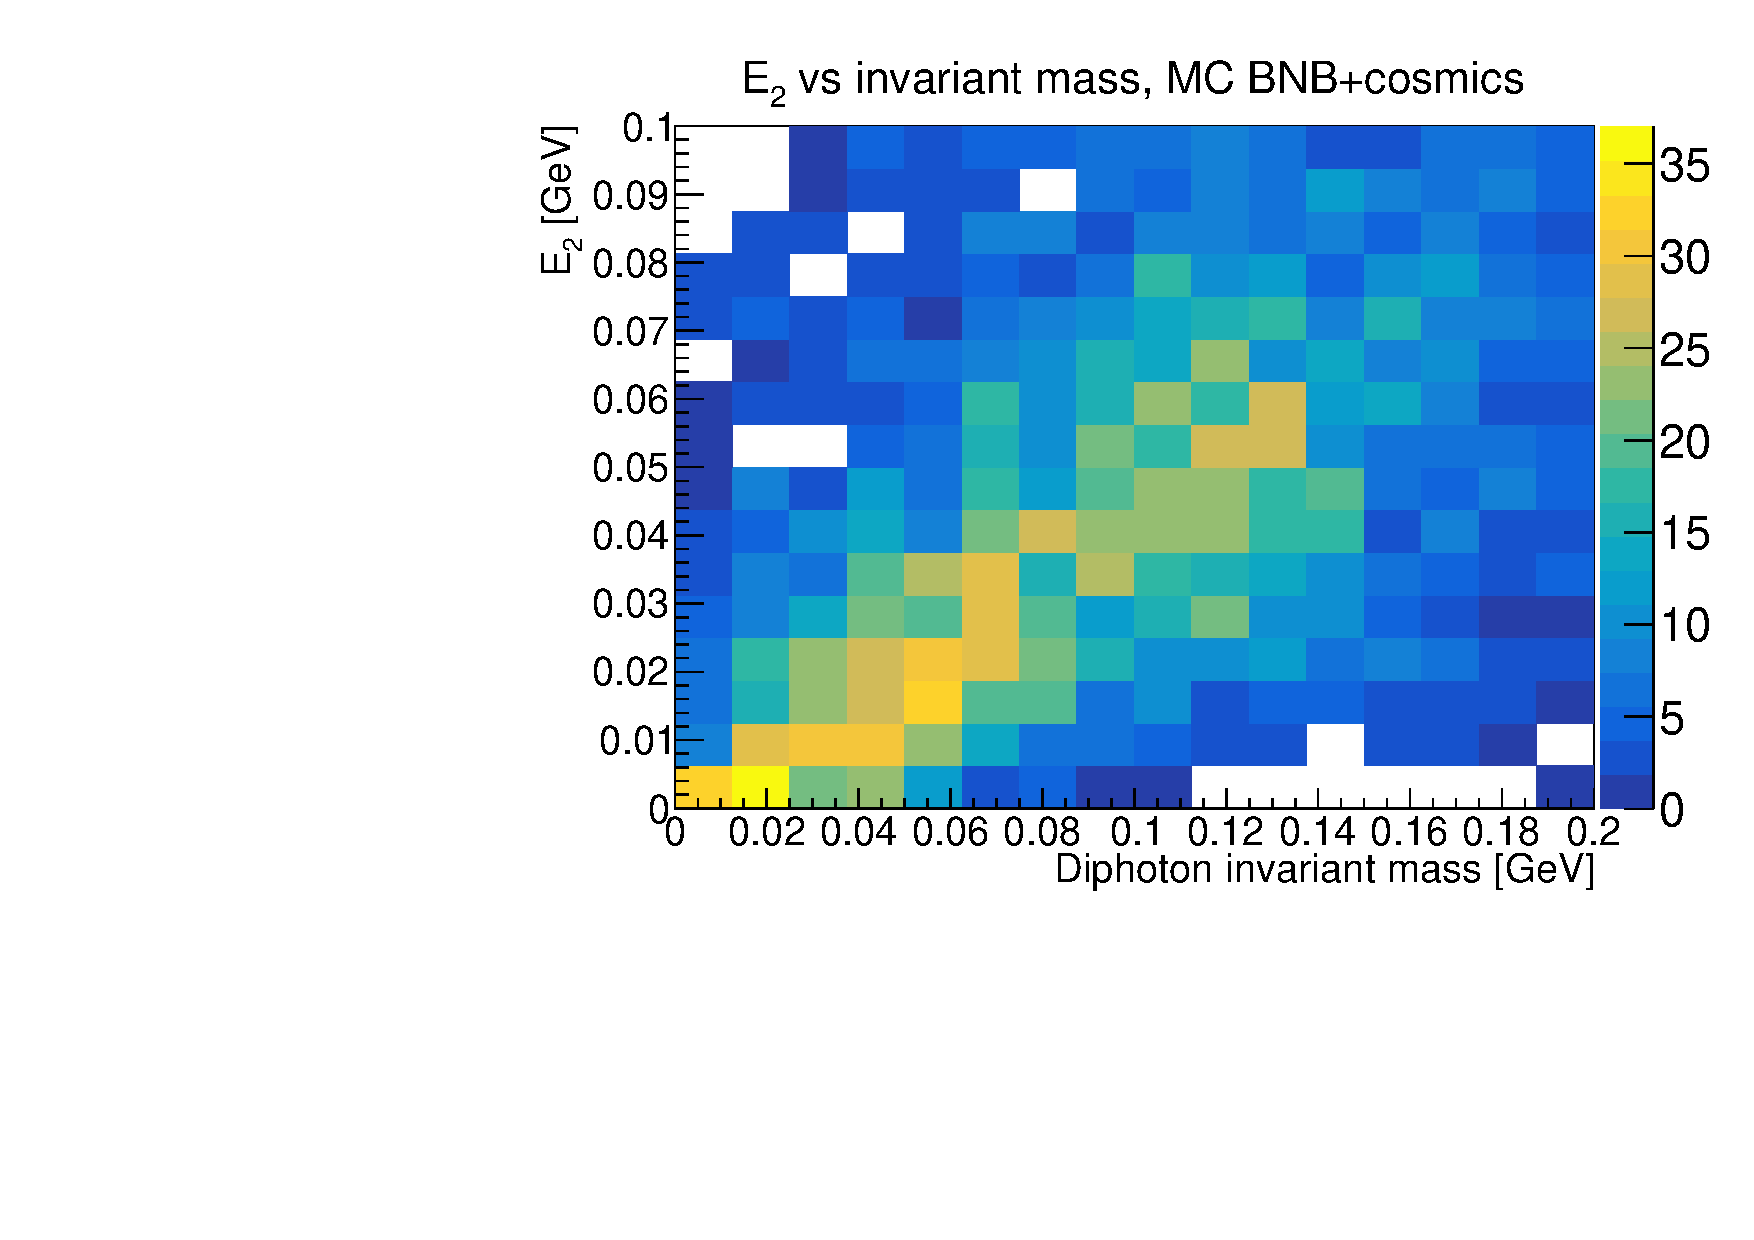
\includegraphics[width=0.99\columnwidth]{figures/MC_mass_E2.pdf}
\end{minipage}
\caption{Left: Distribution of the number of showers for each event, for data (black dots) and Monte Carlo (red boxes). Right: Bi-dimensional distribution of $E_2$ (y-axis) versus the invariant mass (x-axis) in Monte Carlo events.}
\label{fig:mc_mass_e2}
\end{figure}

In some cases a significant amount of energy is missing. For instance, one of the two main showers is missed, and a smaller shower, resulting from noise or from mis-reconstruction of other objects, is taken as one of the decay products of the $\pi^0$. The right plot in Figure \ref{fig:mc_mass_e2} shows the bi-dimensional distribution of the invariant mass ($x$ axis) versus $E_2$ ($y$ axis) for Monte Carlo events. As it is possible to see, a significant amount of events has small $E_2$ and small mass. Thus, to take into account this effect and remove events with one shower badly or mis-reconstructed, the second most energetic shower is required to have reconstructed energy larger than 30~MeV.

The final peak after the selection is shown in Figure \ref{fig:pi0_mass_peak}. The two histograms, for data and Monte Carlo, are fitted through a binned maximum likelihood (ML) fit with a crystal ball function, which consists of a Gaussian core, $C^1$-matched with a power-law right tail. The fit result, for what concerns the core is:
\[ \text{Data:} \quad \mu = 133 \pm 7~\text{MeV}, \quad \sigma = 47 \pm 5~\text{MeV} \]
\[ \text{Monte Carlo:} \quad \mu = 119 \pm 2~\text{MeV}, \quad \sigma = 51 \pm 2~\text{MeV} \]

The two results are significantly close to the nominal mass of 135~MeV, and shows a relatively good agreement between data and Monte Carlo. However, the discrepancy is significant and requires more investigation, in order to be understood completely.

\begin{figure}[htbp]
\centering
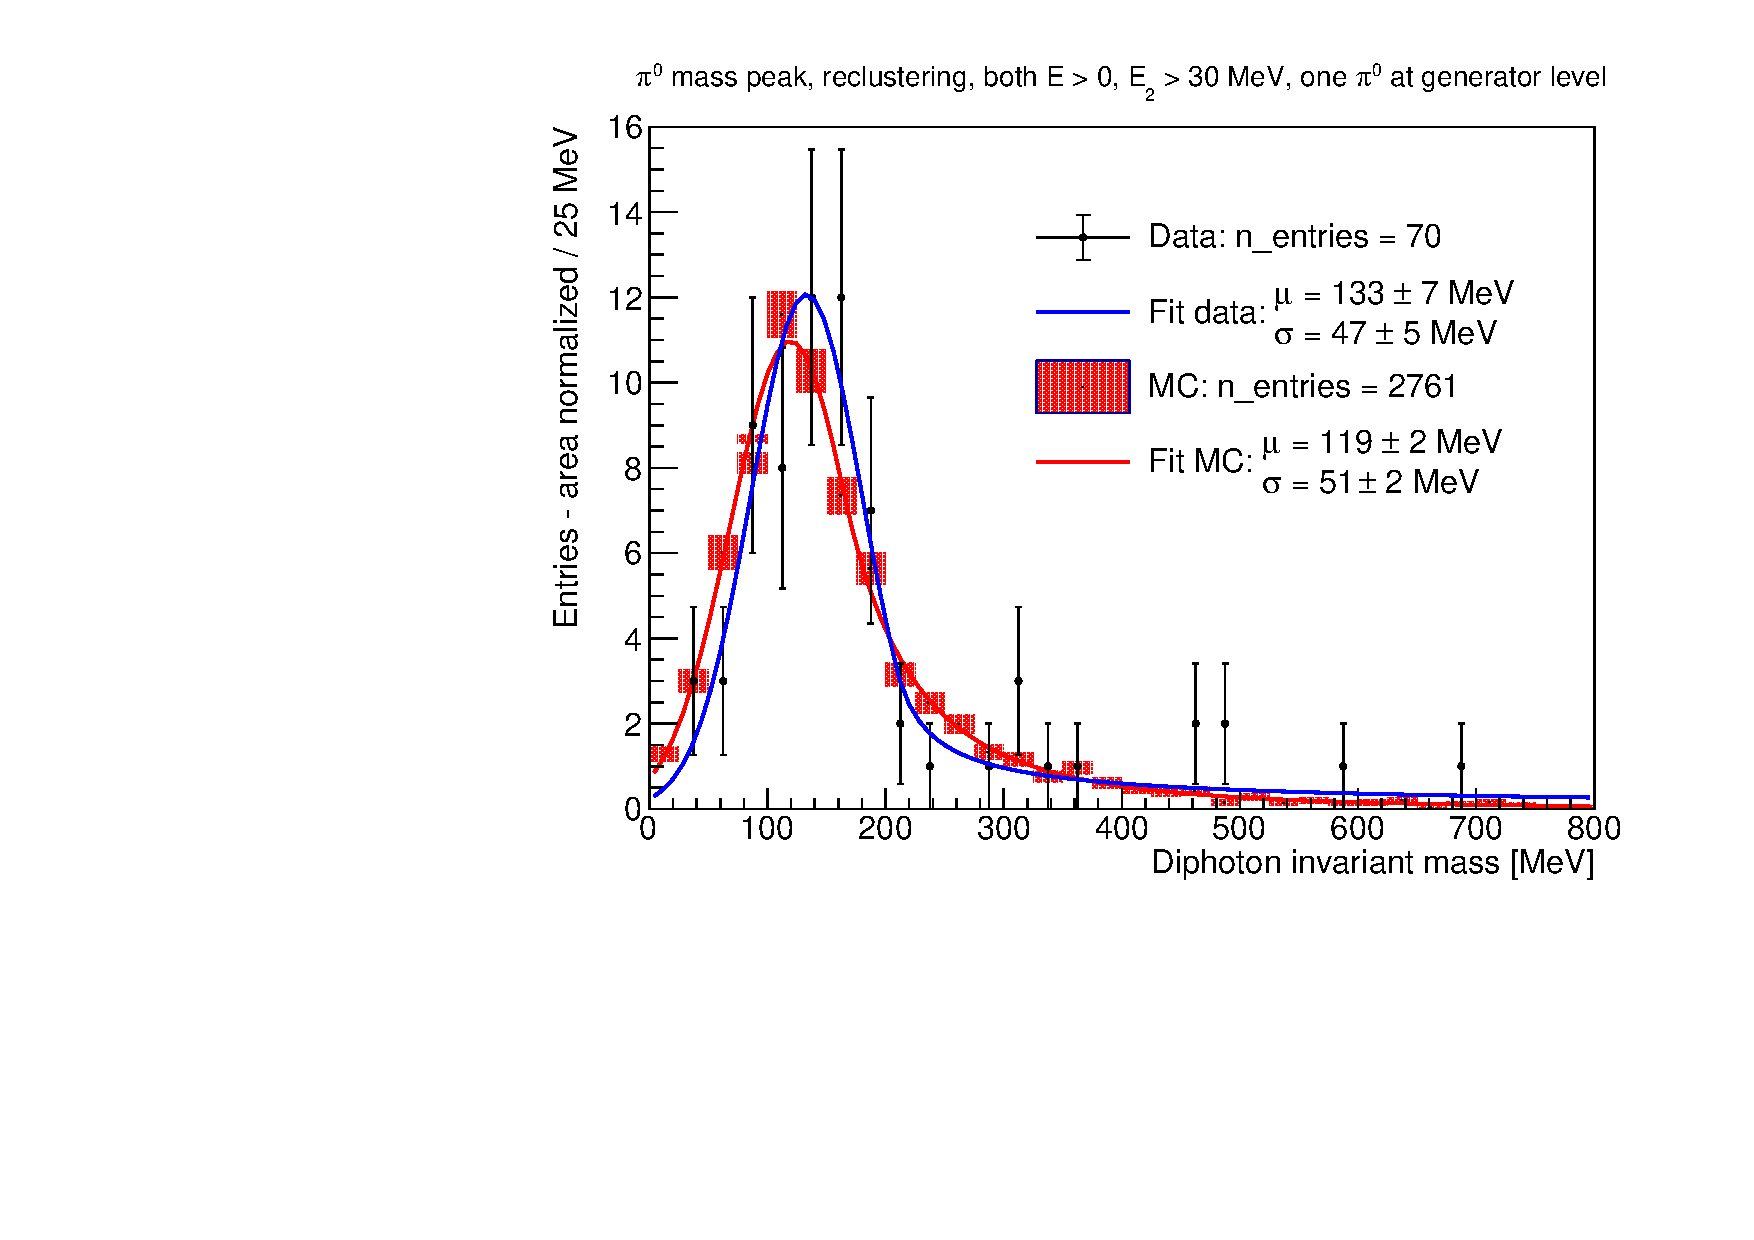
\includegraphics[width=0.65\textwidth]{figures/pi0_mass_peak_final.pdf}
\caption{Di-photon invariant mass distribution for data and Monte Carlo. The two lines show the crystal ball functions as obtained from the ML fit to the two histograms.} 
\label{fig:pi0_mass_peak}
\end{figure}

\subsection{Hadronic Energy Reconstruction}
\todo{Hadronic Energy Reconstruction}
To be included in future iterations.

\subsection{Single proton energy reconstruction and calibration}\label{sec:protonenergy}
Proton energy reconstruction is obtained converting the reconstructed track length $L$ into deposited energy using the proton stopping power in liquid argon, as tabulated in \cite{pstar}. Liquid argon density $\rho_{\mathrm{LAr}}$ is assumed to be constant at 1.379~g/ml. Figure \ref{fig:proton} shows the proton kinetic energy as a function of the range of the proton in liquid argon (measured as $L \times \rho_{\mathrm{LAr}}$) .

\begin{figure}[htbp]
\centering
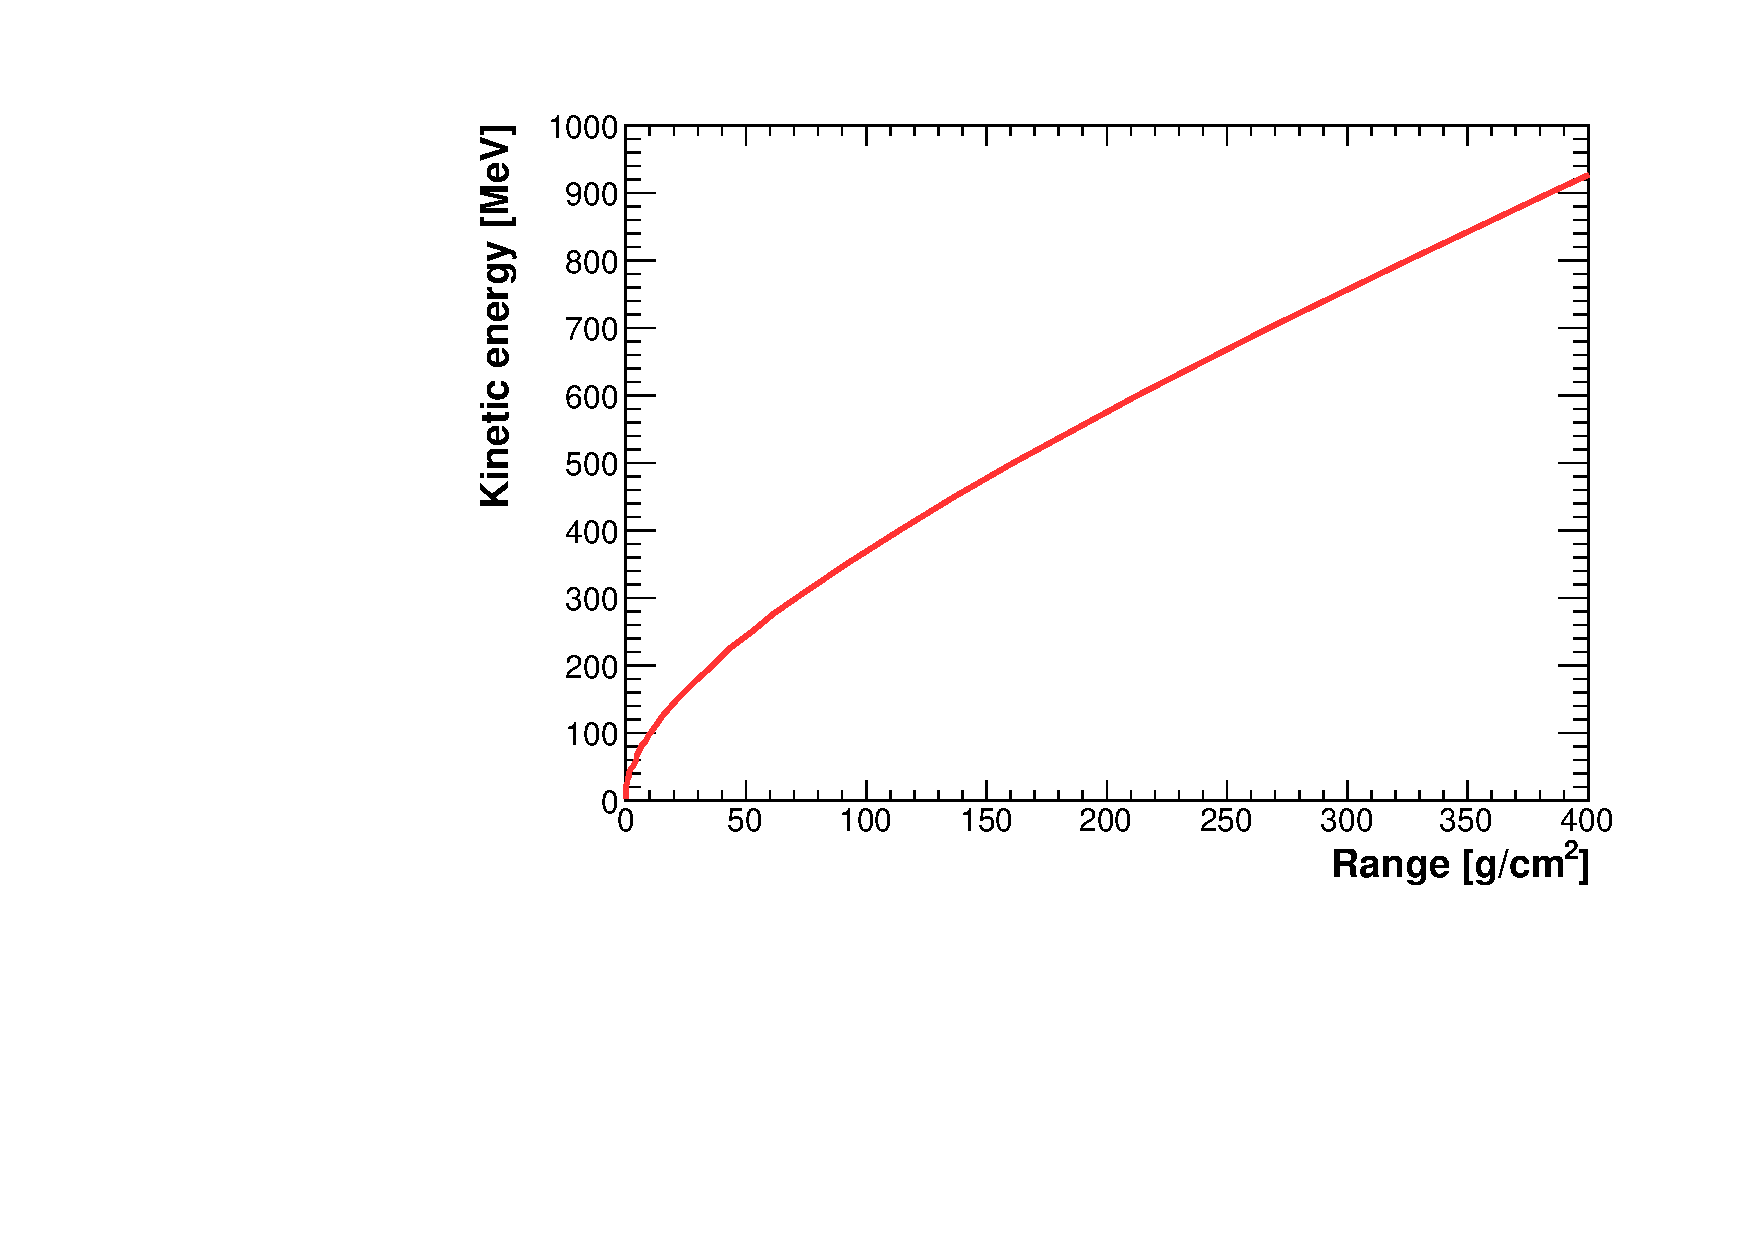
\includegraphics[width=0.65\textwidth]{figures/proton.pdf}
\caption{Proton kinetic energy as a function of the range of the proton in liquid argon. Values are taken from \cite{pstar}.} 
\label{fig:proton}
\end{figure}

The calibration constant has been obtained comparing the reconstructed energy of the proton with the true kinetic energy of the proton, in a CC $\nu_{e}$ sample with only one proton in the final state. The true proton and the reconstructed tracks are required to be fully contained within the fiducial volume. Since protons are not MIPs, in the case of two or more tracks (\emph{split tracks}) associated to the same proton, the reconstructed length of the tracks has been summed before calculating the corresponding kinetic energy.
Figure \ref{fig:pcalib} shows the calibration slope necessary to convert the proton reconstructed energy $E_{reco}^{p}$ into true proton kinetic energy $E_{true}^{p}$. For each bin of the true proton energy, the most probable value of the corresponding proton reconstructed energy has been obtained with a Gaussian fit around the peak of the distribution. A linear fit of the data points gives:
\begin{equation}
E_{reco}^{p} = 0.99~E^{p}.
\end{equation}

\begin{figure}[htbp]
\centering
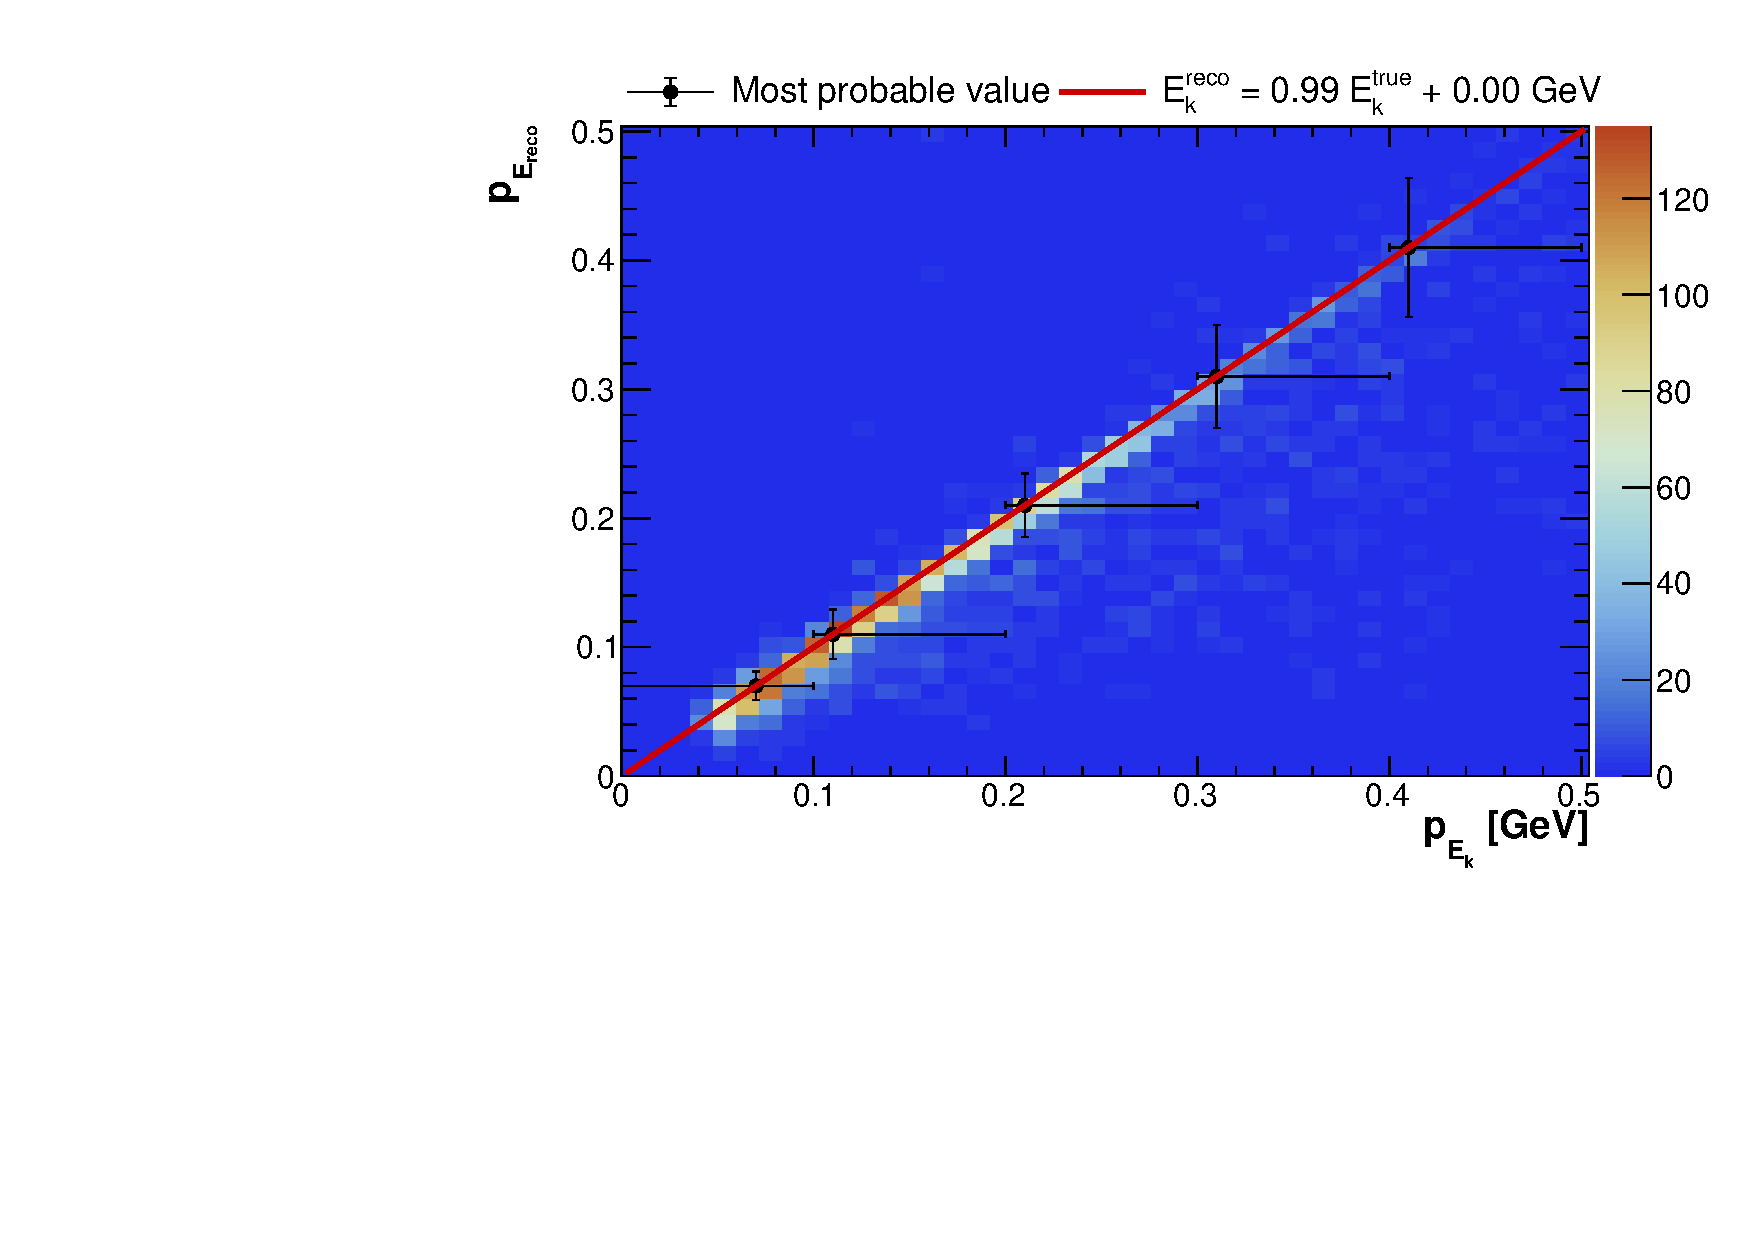
\includegraphics[width=0.65\columnwidth]{figures/pcalib.pdf}
\caption{Bi-dimensional histogram of true proton energy $E^{p}$ vs. reconstructed proton energy $E_{reco}^{p}$. Black points are obtained measuring the most probable value of the $E_{reco}^{p}$ distribution for each $E^{p}$ bin.}
\label{fig:pcalib}
\end{figure}


% \subsubsection{Neutrino Produced Hadronic Energy Reconstruction}

\subsection{Neutrino Energy Reconstruction}
\todo{Neutrino Energy Reconstruction}
To be included in future iterations.

